\documentclass[review]{elsarticle}
\DeclareGraphicsExtensions{.pdf,.gif,.jpg}

%Packages Used
\usepackage{amssymb} %Allows to use Rho and other math symbols
\usepackage{graphicx}%Includes images/figures in the document
%\usepackage{lineno}%for the numbering of lines
%\usepackage{Iscape} %for use landscape pages in the document 
\usepackage{natbib}%used for the elstartd documentclass
\usepackage{subfig} %Use of subfigures


\usepackage{lineno,hyperref}
\modulolinenumbers[5]

%\journal{Journal of \LaTeX\ Templates}




%New command
\newcommand{\cfert}{$\mathrm{CFE}_{RT}$}
\newcommand{\cferts}{$\mathrm{CFE}_{RT}~$}
\newcommand{\cfea}{$\mathrm{CFE}_{AC}$}
\newcommand{\cfeast}{$\mathrm{CFE}_{RT}~$}
\newcommand{\cfed}{$\mathrm{CFE}_{d'}$}
\newcommand{\cfeds}{$\mathrm{CFE}_{d'}~$}
\newcommand{\dprimw}{$d^{\prime}~$}
\newcommand{\R}{${\rho}$}
\newcommand{\Rs}{${\rho}$\space}
\newcommand{\<}{${<}$}


\renewcommand{\emph}{\textbf}   %for underlining and itaicizing 



%%%%%%%%%%%%%%%%%%%%%%%
%% Elsevier bibliography styles
%%%%%%%%%%%%%%%%%%%%%%%
%% To change the style, put a % in front of the second line of the current style and
%% remove the % from the second line of the style you would like to use.
%%%%%%%%%%%%%%%%%%%%%%%

%% Numbered
%\bibliographystyle{model1-num-names}

%% Numbered without titles
%\bibliographystyle{model1a-num-names}

%% Harvard
%\bibliographystyle{model2-names.bst}\biboptions{authoryear}

%% Vancouver numbered
%\usepackage{numcompress}\bibliographystyle{model3-num-names}

%% Vancouver name/year
%\usepackage{numcompress}\bibliographystyle{model4-names}\biboptions{authoryear}

%% APA style
%\bibliographystyle{model5-names}\biboptions{authoryear}

%% AMA style
%\usepackage{numcompress}\bibliographystyle{model6-num-names}

%% `Elsevier LaTeX' style
\bibliographystyle{elsarticle-num}
%%%%%%%%%%%%%%%%%%%%%%%


\setcounter{secnumdepth}{-1}
\begin{document}

\begin{frontmatter}

\title{Deeply Supervised U-Net for Mass Segmentation in Digital Mammograms}
\author{N Ravitha Rajalakshmi}
\author{Nikhil Ramesh}
\date{}
%\tnotetext[mytitlenote]{Fully documented templates are available in the elsarticle package on \href{http://www.ctan.org/tex-archive/macros/latex/contrib/elsarticle}{CTAN}.}

%% Group authors per affiliation:
%\author{AUTHORNAME\fnref{myfootnote}}
%\address{Radarweg 29, Amsterdam}
%\fntext[myfootnote]{Since 1880.}


%% or include affiliations in footnotes:
%\author[mymainaddress,mysecondaryaddress]{Elsevier Inc}
%\ead[url]{www.elsevier.com}

%\author[mysecondaryaddress]{Global Customer Service\corref{mycorrespondingauthor}}
%\cortext[mycorrespondingauthor]{Corresponding author}
%\ead{support@elsevier.com}

%\address[mymainaddress]{1600 John F Kennedy Boulevard, Philadelphia}
%\address[mysecondaryaddress]{360 Park Avenue South, New York}


%Abstract
\begin{abstract}
Mass detection is a critical process in the review of mammograms. The shape and texture of the masses are key indicators in the prognosis of the medical condition. Hence, semantic segmentation is found to be useful in this context rather than mere object detection (or) localization. The main challenges involved in the semantic segmentation of masses in mammograms include (1) higher signal to noise ratio (SNR) (2) indiscernible mass boundaries and (3) more false positives due to significant overlap in the intensities between the normal parenchymal regions and masses. To address these challenges, we propose DS U-Net (Deeply Supervised U-net model) coupled with Dense CRF (Conditional Random Fields). Most of the state-of-art approaches for semantic segmentation uses Encoder - Decoder based model. Encoder captures low-level features such as presence of mass in multiple stages. Decoder path provides the precise segmentation in multiple stages by combining the intermediate results from the encoder at each stage through skip connections. The resulting segmentation map lack the ability of capturing the non-conspicuous and spiculated mass boundaries. In the proposed work, deep supervision is integrated with popular Encoder - Decoder model (U-net) to monitor the low level features for proper attention of the boundaries of suspicious regions and higher level features for accurate segmentation of the entire mass. The final segmentation map is obtained by fusing the intermediate outputs with the final output using learnable weights. The resulting segmentation map is fine tuned using Dense CRF to enhance the edges. We evaluated the model on two publicly available benchmark datasets CBIS-DDSM and INBREAST. DS U-Net with DenseCRF provides Dice score of 84\% for CBIS-DDSM and 82.6\% for INBREAST.  
\end{abstract}

%Keyword
\begin{keyword}
 Mass Segmentation, Deep Supervision, Mammograms, Conditional Random Fields
\end{keyword}

\end{frontmatter}

%\linenumbers

\section{I Introduction }

Global Cancer Observatory Database released in 2018 reports that Breast cancer is contributing to over 25.4\% of all the new cases diagnosed \citep{}[1].  Henceforth, Governments are conducting screening programmes to curb the disease. Mammograms are widely adopted as  the primary screening tool to diagnose breast cancer. A mammogram is an x-ray image of the breast which captures the changes in the breast tissue. Presence of masses and microcalcifications in the mammogram characterize the disease. The detection of these regions in mammograms are difficult as their pixel intensities often correlate with normal tissue. 

CAD (computer aided detection) tools uses digitally captured images of the mammogram and employs artificial intelligence based techniques to detect suspicious regions in them. CAD has been constantly evolving with the advent of new techniques in the domain to provide accurate results. With the recent success of deep neural networks in most of the vision oriented challenges, they are been explored for medical diagnosis. 

The main contributions of the work include:
\begin{enumerate}
   \item We propose Deep Supervised U-net for mass segmentation in whole mammograms to monitor the attention of the intermediate layers.  Encoder layers are directed towards proper attention of the mass boundaries and decoder layers are directed towards proper attention of the mass regions. This reduces false positives and leads to faster convergence.
   \item We use a learnable fusion layer to fuse the output of the attention layers with the last layer to produce the final segmentation result.
   \item We employ Combined loss function for the fusion layer to address the class imbalance problems (mass usually occupies a smaller percentage of the entire image). This loss penalizes the false positives more.
     \item Unlike other works, we use preprocessing and post processing steps to improve the accuracy of the model. CLAHE is used to enhance the contrast of the input mammogram images and Dense CRF is used to recover the mass boundaries which got smoother due to the rigorous downsampling.
\end{enumerate}

\section{II Method }
\begin{enumerate}
\item \textbf {Overview} 
The proposed model employs an end-to-end framework for mass segmentation in mammograms.  The input images are processed through Contrast limited Adaptive histogram equalization technique (CLAHE).  The resulting images are then normalized and resized to 256*256 to train Deep Supervised U-net. During the testing phase, resulting softmax probabilities of DS U-net are further refined using Dense CRF for  definite edges. Fig 2 shows the various components involved in the proposed work.

\item \textbf {Preprocessing} \newline
Preprocessing is often neglected when deep neural networks are used for segmentation. But, mammogram images exhibit high SNR and hence the detection becomes infeasible without proper preprocessing. Histogram equalization and its variants are found to be efficient for mammogram images[10][11]. Hence, CLAHE has been adopted to improve the local contrast of the image. The algorithm is also found to improve the edge boundaries in each region of the image. Fig 3 shows the sample images from INBREAST and CBIS-DDSM which are enhanced using CLAHE.

\item \textbf {Deep Supervised U-net} \newline
Deep Supervised nets [6][7] brings in transparency to the intermediate hidden layers in deep neural networks by considering their error factor with respect to the ground truth in the training objective criterion. It has improved robustness of the neural networks in both segmentation and classification[6]. In segmentation, the output of intermediate layers are upsampled and compared with ground truth to quantize their error margin.  U-net[9] has become the de-facto standard for biomedical image segmentation. It employs an encoder decoder based architecture. Encoder consists of convolution layers for retrieving contextual information and pooling layers to downsample the images. Downsampling facilitates retrieval of higher level contextual information. Unet has symmetrical decoder path which upsamples the information to get the spatial context of the retrieved information. Skip connections are pathways which carry the spatial information from encoder to decoder pathway. Many works have further improved U-net by varying upsampling techniques , using mixed pooling techniques (or) modifying the loss functions. Due to the symmetricity of the encoder and decoder , Unet always produces smoother segmentation map. Hence, DS U-net is used to obtain finer boundaries and eliminate the false positives. The proposed work has extended over the idea of Chen et al[8] and Mishra et al[9] to use different intermediate layers of segmentation network to focus on the boundaries and regions simultaneously. Fig 4 shows the complete architecture of the DS U-net.

%\begin{figure}[t]
%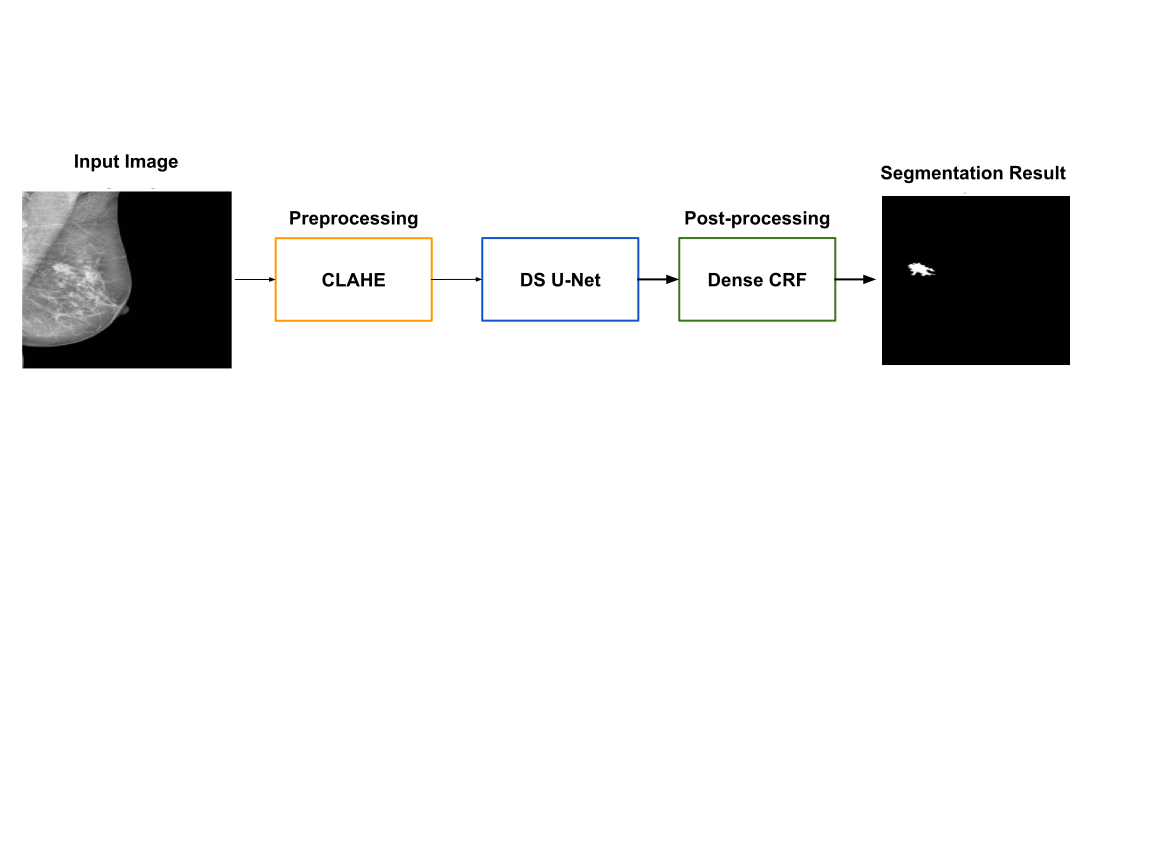
\includegraphics[width=\textwidth]{fig2_vector}
%\centering
%\end{figure}

\end{enumerate}

\section{Front matter}

The author names and affiliations could be formatted in two ways:
\begin{enumerate}[(1)]
\item Group the authors per affiliation.
\item Use footnotes to indicate the affiliations.
\end{enumerate}
See the front matter of this document for examples. You are recommended to conform your choice to the journal you are submitting to.

\section{Bibliography styles}

There are various bibliography styles available. You can select the style of your choice in the preamble of this document. These styles are Elsevier styles based on standard styles like Harvard and Vancouver. Please use Bib\TeX\ to generate your bibliography and include DOIs whenever available.

Here are two sample references: \cite{Feynman1963118,Dirac1953888}.

\section*{References}

\bibliography{mybib}

\end{document}
